\documentclass{tufte-handout}
\usepackage{graphicx}
\usepackage{amsmath}
\graphicspath{ {./img/} }

\title{Basics of Digital Imaging}
\author{Andr\'es Ponce}

\begin{document}
\maketitle
\begin{abstract}
	Digital imaging looks at individual pixel values in (x, y) format.
\end{abstract}

\section{Introduction}
An \textbf{image} is an array of values that describe the color at a point.

We sometimes want to store a series of images, maybe from some video stream.
We have to think of that as \textbf{sampling}\footnote{\textbf{Sampling} refers to 
getting the values at discrete points in the spatial/temporal domains.} 
the environment $x$ times per second.

Since there are only a finite set of values that the image can take digitally,
we might need to \textbf{quantize} the result. Quanitization means that we assign
a discrete set of values to numbers which originally might not be discrete.

\textbf{Image zooming} refers to showing a part of the image at a different size.
How do we calculate the values of the new images? There are a couple methods.

The first is a \textbf{nearest neighbor} method, where we interpolate the values 
of the surrounding pixels. This means that an individual pixel's value will be 
a linear combination of surrounding pixels. The way we determine the nearest 
pixels would be comparing the one in the image with the one in the zoomed 
image.

\begin{marginfigure}
	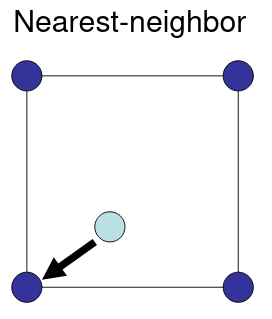
\includegraphics[scale=0.3]{nn}
	\caption{The nearest neighbor method will assign the pixel the same value
			as the closest pixel.}
\end{marginfigure}

Other methods, such as \textbf{bilinear} and \textbf{trilinear} take some combination
of surrounding pixels.

\subsection{Geometric Transformations}
Geometric transformations change the spatial arrangement of pixels but do not really
change the relationship between the pixels themselves. In \textbf{affine} 
transformations any straight line and parallelism are preserved.

The usual way that this is done involves finding the mapping in reverse direction.
We call this an \textbf{inverse mapping}. This mapping involves starting at the transformed
image coordinates and trying to find the mapping to go to the original image.

\[ 
	\begin{bmatrix}	
	x \\
	y \\
	1
	\end{bmatrix}
= A^{-1}
	\begin{bmatrix}
	x' \\
	y' \\
	z' 
	\end{bmatrix}
\]

\section{Intensity Transformations}
There are different methods we could use for image enhancement, and some involve the 
\textbf{spatial domain}, or the pixels themselves, and the \textbf{frequency domain},
which involves finding the Fourier Transform of the images.

An example on a greyscale image is textbf{thresholding}, where we assign 0 to a pixel
$0$ if the pixel's intensity is above a certain value and 0 otherwise. The final result
is a photo with only full white or full black pictures.

A \textbf{histogram} plots the total number of pixels $n_{k}$ with an intensity level
of $k$, $r_{k}$. The resulting graph resembles a bar graph containing the pixel 
intensity values.
\end{document}
